\documentclass[]{article}
\usepackage[letterpaper]{geometry}
\usepackage[utf8]{inputenc}
\usepackage{fancyhdr}
\usepackage{graphicx}

\geometry{headheight = 5 cm,
          left=2 cm,
          right=2 cm,
          top=4.35 cm}

\pagestyle{fancy}

\lhead{
\includegraphics[height=1.5cm]{imagenes/isotipo}}
\rhead{\sc\small Universidad Técnica Federico Santa María\\Campus Santiago San Joaquín\\Optimización\\2$^\circ$ semestre 2017}

\cfoot{\thepage}

\renewcommand{\headrulewidth}{0pt}

\title{Laboratorio 1}

\author{Profesor: Carlos Castro\\ 
        Integrantes: Giorgio Pellizzari y Gabriel Valenzuela}
\date{Octubre 2017}

\begin{document}

\maketitle
\thispagestyle{fancy}

\section{Pregunta 1:}

Para este problema se decidió considerar que los viajes sólo se realizarán desde Ciudad de México a sus destinos y que estos regresarán directo a Ciudad de México ya que no se tiene claridad de que el modelamiento completo de esta problema resulte en un problema lineal.

\subsection{Función objetivo:}
La función asociada al costo que se busca optimizar es la que se describe a continuación:
$$f(x_i,y,z_i)= \sum_{i=Oaxaca}^{Tabasco}x\cdot{}P_{ci}+y\cdot{}P_a+\sum_{i=Oaxaca}^{Tabasco}{P_t\cdot{}Z_i}$$

\par Donde:
\begin{itemize}
    \item $x$ corresponde a la cantidad de camiones.
    \item $y$ corresponde a la cantidad de aviones.
    \item $z_i$ corresponde a toneladas de carga en camiones destinados a la ciudad $i$.
    \item $P_{ci}$ corresponde al costo de rentar un camión para $i$ ciudad.
    \item $P_a$ corresponde al costo de rentar un avión, y equivale a 450000.
    \item $P_t$ corresponde al costo por tonelada de carga en camión, y equivale a 8000.
\end{itemize}

Esto se plantea de tal forma que sólo participan aquellas variables que influyen en el costo total.

\subsection{Restricciones:}
La función anterior descrita queda sujeta a las siguientes condiciones:

$$0\leq \sum_{i=Oaxaca}^{Tabasco}Z_i \leq \sum_{i=Oaxaca}^{Tabasco}C_c\cdot x_i$$

Donde $C_c$ es la capacidad de carga de un camión, que equivale a $18 [Ton]$. Esta restricción muestra que el total de carga de los camiones no puede ser superior a su capacidad.

$$0\leq \sum_{i=Oaxaca}^{Tabasco}W_i \leq C_a\cdot y$$

Donde $W_i$ corresponde a toneladas de carga en aviones destinados a la ciudad $i$ y $C_a$ a la capacidad de carga de un avión, que equivale a $54 [Ton]$. Esta restricción muestra que el total de carga de los camiones no puede ser superior a su capacidad.

$$0 \geq \sum_{i=Oaxaca}^{Tabasco}{W_i+Z_i} \geq \sum_{i=Oaxaca}^{Tabasco}{\left(\sum_{j=Material}^{Carne}{\left(\sum_{k=Camion}^{Avion}{\left(C_{ijk}\right)}\right)}\right)}$$

Donde $C_{ijk}$ corresponde a la cantidad de carga del recurso $j$ para la ciudad $i$ en el medio de transporte $k$. Esta restricción denota que la cantidad de carga entre aviones y camiones debe cumplir con los requisitos diarios de recursos para cada ciudad.

Posteriormente, y tras analizar los tiempos que demoran en llegar los camiones y aviones a cada ciudad, se comprobó la viabilidad de transportar ciertos productos a las ciudades, concluyendo así con el siguiente resultado:

\begin{table}[!htb]
    \centering
    \begin{tabular}{|c|c|c|c|}\hline %Columnas centradas con un separador en la primera. Podemos alinear a la izq o der con l o r
        \textbf{Ciudades} & \textbf{Oaxaca} & \textbf{Chiapas} & \textbf{Tabasco}\\ \hline
        Ciudad de México & 5.8/0.5 & 12.5/1 & 18.8/0.9 \\ \hline
    \end{tabular}
\end{table}

Luego de estos resultados se obtienen las siguientes restricciones para cumplir con los tiempos de los recursos:

$$C_{chiapas-lacteos-camion}=0$$
$$\sum_{j=Lacteos}^{Carnes}C_{tabasco-j-camion}=0$$

Finalmente se tiene la siguiente condición para la cantidad de horas que puede usarse un camión mientras este está arrendado:

$$P_{c-Oaxaca}=150000$$

$$\sum_{i=Chiapas}^{Tabasco}P_{ci}=300000$$

Esto producto de que sera necesario arrendar durante $48$ horas para los viajes en camión hacia Chiapas y Tabasco.



\section{Pregunta 2:}

\subsection{Parte A:}

Se presenta el siguiente modelo para resolver el problema propuesto:

\begin{itemize}
    
\item $R_i$: Cantidad de anuncios en el medio $i$.

\item Función a Maximizar:

$$Zmax(R_1,R_2)=R_1\cdot 3400 + R_2\cdot 7600$$

\item Restricciones:
$$R_1 , R_2 \geq 0$$
$$R_1\cdot 210 + R_2\cdot 566 \leq 20048$$
$$R_1\cdot1,1 \leq R_2$$
$$R_1 \leq 20$$
$$R_2 \leq 37$$
\end{itemize}

\subsubsection{Simplex:}

\begin{table}[!htb]
    \centering
    \begin{tabular}{c|c|c|c|c|c|c|c|c|c} %Columnas centradas con un separador en la primera. Podemos alinear a la izq o der con l o r
         & & $R_1$ & $R_2$ & $S_1$ & $S_2$ & $S_3$ & $S_4$ & & \\ \hline
        Basis & $c_j$ & 3400 & 7600 & 0 & 0 & 0 & 0 & $b_i$ & $\frac{b_i}{a_{ij}}$\\ \hline
        $S_1$ & 0 & 210 & \textbf{566} & 1 & 0 & 0 & 0 & 20048 & $\textbf{35.42}$\\ \hline
        $S_2$ & 0 & 1.1 & \textbf{-1} & 0 & 1 & 0 & 0 & 0 & 0\\ \hline
        $S_3$ & 0 & 1 & \textbf{0} & 0 & 0 & 1 & 0 & 20 & --\\ \hline
        $S_4$ & 0 & 0 & \textbf{1} & 0 & 0 & 0 & 1 & 37 & 37\\ \hline
        $Z_j$ & & 0 & 0 & 0 & 0 & 0 & 0 & 0 & \\
        $C_j-Z_j$ & & 3400 & \textbf{7600} & 0 & 0 & 0 & 0 & & \\
    \end{tabular}
\end{table}

\begin{table}[!htb]
    \centering
    \begin{tabular}{c|c|c|c|c|c|c|c|c|c} %Columnas centradas con un separador en la primera. Podemos alinear a la izq o der con l o r
         & & $R_1$ & $R_2$ & $S_1$ & $S_2$ & $S_3$ & $S_4$ & & \\ \hline
        Basis & $c_j$ & 3400 & 7600 & 0 & 0 & 0 & 0 & $b_i$ & $\frac{b_i}{a_{ij}}$\\ \hline
        $R_2$ & 7600 & \textbf{0.37} & 1 & 0 & 0 & 0 & 0 & 35.42 & 95.47\\ \hline
        $S_2$ & 0 & \textbf{1.47} & 0 & 0 & 1 & 0 & 0 & 35.42 & 24.08\\ \hline
        $S_3$ & 0 & \textbf{1} & 0 & 0 & 0 & 1 & 0 & 20 & \textbf{20}\\ \hline
        $S_4$ & 0 & \textbf{-0.37} & 0 & 0 & 0 & 0 & 1 & 1.58 & --\\ \hline
        $Z_j$ & & 2819.79 & 7600 & 13.43 & 0 & 0 & 0 & 269195.76 & \\
        $C_j-Z_j$ & & \textbf{580.21} & 0 & -13.43 & 0 & 0 & 0 & & \\
    \end{tabular}
\end{table}

\begin{table}[!htb]
    \centering
    \begin{tabular}{c|c|c|c|c|c|c|c|c|c} %Columnas centradas con un separador en la primera. Podemos alinear a la izq o der con l o r
         & & $R_1$ & $R_2$ & $S_1$ & $S_2$ & $S_3$ & $S_4$ & & \\ \hline
        Basis & $c_j$ & 3400 & 7600 & 0 & 0 & 0 & 0 & $b_i$ & $\frac{b_i}{a_{ij}}$\\ \hline
        $R_2$ & 7600 & 0 & 1 & 0 & 0 & -0.37 & 0 & 28 & --\\ \hline
        $S_2$ & 0 & 0 & 0 & 0 & 1 & -1.47 & 0 & 6 & --\\ \hline
        $R_1$ & 3400 & 1 & 0 & 0 & 0 & 1 & 0 & 20 & --\\ \hline
        $S_4$ & 0 & 0 & 0 & 0 & 0 & 0.37 & 1 & 9 & --\\ \hline
        $Z_j$ & & 3400 & 7600 & 13.43 & 0 & 580.21 & 0 & 280800 & \\
        $C_j-Z_j$ & & 0 & 0 & -13.43 & 0 & -580.21 & 0 & & \\
    \end{tabular}
\end{table}
Finalmente se obtuvieron los valores de 20 para $R_1$ y 28 para $R_2$
\newpage

\subsubsection{Metodo gráfico}

\begin{figure}[h] 
\centering
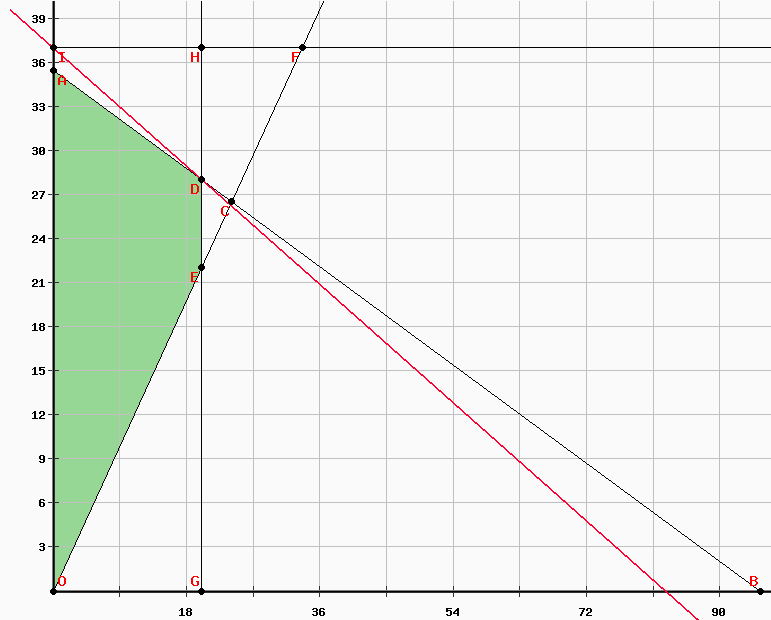
\includegraphics[scale=0.4]{grafico.png}
\end{figure}


\newpage
\subsection{Parte B:}

Se presenta el siguiente modelo para resolver el problema propuesto:

\begin{itemize}
    
\item $R_i$: Cantidad de anuncios en el medio $i$.

\item Función a Maximizar:

$$Zmax(R_1,R_2,R_3,R_4)=R_1\cdot 3400 + R_2\cdot 7600 R_3\cdot33000 + R_4\cdot 20000$$

\item Restricciones:

$$R_1 , R_2 , R_3 , R_4\geq 0$$
$$R_1\cdot 210 + R_2\cdot 566 + R_3\cdot 1800 + R_4\cdot 1480   \leq 24692$$
$$R_1\cdot1,1 \leq R_2$$
$$R_1 \leq 20$$
$$R_2 \leq 37$$
$$R_3 \leq 2$$
$$R_4 \leq 5$$



\end{itemize}

\subsubsection{Simplex:}

\begin{table}[!htb]
    \centering
    \begin{tabular}{c|c|c|c|c|c|c|c|c|c|c|c|c|c} %Columnas centradas con un separador en la primera. Podemos alinear a la izq o der con l o r
         & & $R_1$ & $R_2$ & $R_3$ & $R_4$ & $S_1$ & $S_2$ & $S_3$ & $S_4$ & $S_5$ & $S_6$ & & \\ \hline
        Basis & $c_j$ & 3400 & 7600 & 33000 & 20000 & 0 & 0 & 0 & 0 & 0 & 0 & $b_i$ & $\frac{b_i}{a_{ij}}$\\ \hline
        $S_1$ & 0 & 210 & 566 & \textbf{1800} & 1480 & 1 & 0 & 0 & 0 & 0 & 0 & 24692 & 13.72\\ \hline
        $S_2$ & 0 & 1.1 & -1 & \textbf{0} & 0 & 0 & 1 & 0 & 0 & 0 & 0 & 0 & --\\ \hline
        $S_3$ & 0 & 1 & 0 & \textbf{0} & 0 & 0 & 0 & 1 & 0 & 0 & 0 & 20 & --\\ \hline
        $S_4$ & 0 & 0 & 1 & \textbf{0} & 0 & 0 & 0 & 0 & 1 & 0 & 0 & 37 & --\\ \hline
        $S_5$ & 0 & 0 & 0 & \textbf{1} & 0 & 0 & 0 & 0 & 0 & 1 & 0 & 2 & \textbf{2} \\ \hline
        $S_6$ & 0 & 0 & 0 & \textbf{0} & 1 & 0 & 0 & 0 & 0 & 0 & 1 & 5 & --\\ \hline
        $Z_j$ & & 0 & 0 & 0 & 0 & 0 & 0 & 0 & 0 & 0 & 0 & 0 & \\
        $C_j-Z_j$ & & 3400 & 7600 & \textbf{33000} & 20000 & 0 & 0 & 0 & 0 & 0 & 0 & & \\ 
    \end{tabular}
\end{table}

\begin{table}[!htb]
    \centering
    \begin{tabular}{c|c|c|c|c|c|c|c|c|c|c|c|c|c} %Columnas centradas con un separador en la primera. Podemos alinear a la izq o der con l o r
         & & $R_1$ & $R_2$ & $R_3$ & $R_4$ & $S_1$ & $S_2$ & $S_3$ & $S_4$ & $S_5$ & $S_6$ & & \\ \hline
        Basis & $c_j$ & 3400 & 7600 & 33000 & 20000 & 0 & 0 & 0 & 0 & 0 & 0 & $b_i$ & $\frac{b_i}{a_{ij}}$\\ \hline
        $S_1$ & 0 & 210 & 566 & 0 & \textbf{1480} & 1 & 0 & 0 & 0 & -1800 & 0 & 21092 & 14.25\\ \hline
        $S_2$ & 0 & 1.1 & -1 & 0 & \textbf{0} & 0 & 1 & 0 & 0 & 0 & 0 & 0 & --\\ \hline
        $S_3$ & 0 & 1 & 0 & 0 & \textbf{0} & 0 & 0 & 1 & 0 & 0 & 0 & 20 & --\\ \hline
        $S_4$ & 0 & 0 & 1 & 0 & \textbf{0} & 0 & 0 & 0 & 1 & 0 & 0 & 37 & --\\ \hline
        $R_3$ & 33000 & 0 & 0 & 1 & \textbf{0} & 0 & 0 & 0 & 0 & 1 & 0 & 2 & -- \\ \hline
        $S_6$ & 0 & 0 & 0 & 0 & \textbf{1} & 0 & 0 & 0 & 0 & 0 & 1 & 5 & \textbf{5}\\ \hline
        $Z_j$ & & 0 & 0 & 33000 & 0 & 0 & 0 & 0 & 0 & 33000 & 0 & 66000 & \\
        $C_j-Z_j$ & & 3400 & 7600 & 0 & \textbf{20000} & 0 & 0 & 0 & 0 & -33000 & 0 & & \\ 
    \end{tabular}
\end{table}

\begin{table}[!htb]
    \centering
    \resizebox{16cm}{!}{
    \begin{tabular}{c|c|c|c|c|c|c|c|c|c|c|c|c|c} %Columnas centradas con un separador en la primera. Podemos alinear a la izq o der con l o r
         & & $R_1$ & $R_2$ & $R_3$ & $R_4$ & $S_1$ & $S_2$ & $S_3$ & $S_4$ & $S_5$ & $S_6$ & & \\ \hline
        Basis & $c_j$ & 3400 & 7600 & 33000 & 20000 & 0 & 0 & 0 & 0 & 0 & 0 & $b_i$ & $\frac{b_i}{a_{ij}}$\\ \hline
        $S_1$ & 0 & 210 & \textbf{566} & 0 & 0 & 1 & 0 & 0 & 0 & -1800 & -1480 & 13692 & \textbf{24.19}\\ \hline
        $S_2$ & 0 & 1.1 & \textbf{-1} & 0 & 0 & 0 & 1 & 0 & 0 & 0 & 0 & 0 & --\\ \hline
        $S_3$ & 0 & 1 & \textbf{0} & 0 & 0 & 0 & 0 & 1 & 0 & 0 & 0 & 20 & --\\ \hline
        $S_4$ & 0 & 0 & \textbf{1} & 0 & 0 & 0 & 0 & 0 & 1 & 0 & 0 & 37 & 37\\ \hline
        $R_3$ & 33000 & 0 & \textbf{0} & 1 & 0 & 0 & 0 & 0 & 0 & 1 & 0 & 2 & -- \\ \hline
        $R_4$ & 20000 & 0 & \textbf{0} & 0 & 1 & 0 & 0 & 0 & 0 & 0 & 1 & 5 & --\\ \hline
        $Z_j$ & & 0 & 0 & 33000 & 20000 & 0 & 0 & 0 & 0 & 33000 & 20000 & 166000 & \\
        $C_j-Z_j$ & & 3400 & \textbf{7600} & 0 & 0 & 0 & 0 & 0 & 0 & -33000 & -20000 & & \\ 
    \end{tabular}
    }
\end{table}

\begin{table}[!htb]
    \centering
    \resizebox{16cm}{!}{
    \begin{tabular}{c|c|c|c|c|c|c|c|c|c|c|c|c|c} %Columnas centradas con un separador en la primera. Podemos alinear a la izq o der con l o r
         & & $R_1$ & $R_2$ & $R_3$ & $R_4$ & $S_1$ & $S_2$ & $S_3$ & $S_4$ & $S_5$ & $S_6$ & & \\ \hline
        Basis & $c_j$ & 3400 & 7600 & 33000 & 20000 & 0 & 0 & 0 & 0 & 0 & 0 & $b_i$ & $\frac{b_i}{a_{ij}}$\\ \hline
        $R_2$ & 7600 & \textbf{0.37} & 1 & 0 & 0 & 0 & 0 & 0 & 0 & -3.18 & -2.61 & 24.19 & 65.2\\ \hline
        $S_2$ & 0 & \textbf{1.47} & 0 & 0 & 0 & 0 & 1 & 0 & 0 & -3.18 & -2.61 & 24.19 & \textbf{16.44}\\ \hline
        $S_3$ & 0 & \textbf{1} & 0 & 0 & 0 & 0 & 0 & 1 & 0 & 0 & 0 & 20 & 20\\ \hline
        $S_4$ & 0 & \textbf{-0.37} & 0 & 0 & 0 & 0 & 0 & 0 & 1 & 3.18 & 2.61 & 12.81 & --\\ \hline
        $R_3$ & 33000 & \textbf{0} & 0 & 1 & 0 & 0 & 0 & 0 & 0 & 1 & 0 & 2 & -- \\ \hline
        $R_4$ & 20000 & \textbf{0} & 0 & 0 & 1 & 0 & 0 & 0 & 0 & 0 & 1 & 5 & --\\ \hline
        $Z_j$ & & 0 & 2819.79 & 33000 & 20000 & 0 & 0 & 0 & 0 & 8830.39 & 127.21 & 349850.18 & \\
        $C_j-Z_j$ & & \textbf{580.21} & 0 & 0 & 0 & -13.43 & 0 & 0 & 0 & -8830.39 & -127.21 & & \\ 
    \end{tabular}
    }
\end{table}

\begin{table}[!htb]
    \centering
    \resizebox{16cm}{!}{
    \begin{tabular}{c|c|c|c|c|c|c|c|c|c|c|c|c|c} %Columnas centradas con un separador en la primera. Podemos alinear a la izq o der con l o r
         & & $R_1$ & $R_2$ & $R_3$ & $R_4$ & $S_1$ & $S_2$ & $S_3$ & $S_4$ & $S_5$ & $S_6$ & & \\ \hline
        Basis & $c_j$ & 3400 & 7600 & 33000 & 20000 & 0 & 0 & 0 & 0 & 0 & 0 & $b_i$ & $\frac{b_i}{a_{ij}}$\\ \hline
        $R_2$ & 7600 & 0 & 1 & 0 & 0 & 0 & -0.25 & 0 & 0 & -2.38 & -1.96 & 18.09 & --\\ \hline
        $R_1$ & 3400 & 1 & 0 & 0 & 0 & 0 & 0.68 & 0 & 0 & -2.16 & -1.78 & 16.44 & --\\ \hline
        $S_3$ & 0 & 0 & 0 & 0 & 0 & 0 & -0.68 & 1 & 0 & 2.16 & 1.78 & 3.56 & \textbf{2}\\ \hline
        $S_4$ & 0 & 0 & 0 & 0 & 0 & 0 & 0.25 & 0 & 1 & 2.38 & 1.96 & 18.91 & 9.67\\ \hline
        $R_3$ & 33000 & 0 & 0 & 1 & 0 & 0 & 0 & 0 & 0 & 1 & 0 & 2 & -- \\ \hline
        $R_4$ & 20000 & 0 & 0 & 0 & 1 & 0 & 0 & 0 & 0 & 0 & 1 & 5 & 5\\ \hline
        $Z_j$ & & 3400 & 2819.79 & 33000 & 20000 & 14.12 & 394.43 & 0 & 0 & 7576.03 & -904.16 & 359391.69 & \\
        $C_j-Z_j$ & & 0 & 0 & 0 & 0 & -14.12 & -394.43 & 0 & 0 & -7576.03 & \textbf{904.16} & & \\ 
    \end{tabular}
    }
\end{table}
\newpage
\begin{table}[!htb]
    \centering
    \resizebox{16cm}{!}{
    \begin{tabular}{c|c|c|c|c|c|c|c|c|c|c|c|c|c} %Columnas centradas con un separador en la primera. Podemos alinear a la izq o der con l o r
         & & $R_1$ & $R_2$ & $R_3$ & $R_4$ & $S_1$ & $S_2$ & $S_3$ & $S_4$ & $S_5$ & $S_6$ & & \\ \hline
        Basis & $c_j$ & 3400 & 7600 & 33000 & 20000 & 0 & 0 & 0 & 0 & 0 & 0 & $b_i$ & $\frac{b_i}{a_{ij}}$\\ \hline
        $R_2$ & 7600 & 0 & 1 & 0 & 0 & 0 & -1 & 1.1 & 0 & 0 & 0 & 22 & --\\ \hline
        $R_1$ & 3400 & 1 & 0 & 0 & 0 & 0 & 0 & 1 & 0 & 0 & 0 & 20 & --\\ \hline
        $S_6$ & 0 & 0 & 0 & 0 & 0 & 0 & -0.38 & 0.56 & 0 & 1.22 & 1 & 2 & --\\ \hline
        $S_4$ & 0 & 0 & 0 & 0 & 0 & 0 & 1 & -1.1 & 1 & 0 & 0 & 15 & --\\ \hline
        $R_3$ & 33000 & 0 & 0 & 1 & 0 & 0 & 0 & 0 & 0 & 1 & 0 & 2 & -- \\ \hline
        $R_4$ & 20000 & 0 & 0 & 0 & 1 & 0 & 0.38 & -0.56 & 0 & -1.22 & 0 & 3 & --\\ \hline
        $Z_j$ & & 3400 & 2819.79 & 33000 & 20000 & 13.51 & 48.65 & 508.65 & 0 & 8675.68 & 0 & 361200 & \\
        $C_j-Z_j$ & & 0 & 0 & 0 & 0 & -13.51 & -48.65 & -508.65 & 0 & -8675.68 & 0 & & \\ 
    \end{tabular}
    }
\end{table}
\newpage
Dado que siguen habiendo valores negativos no se pudo determinar un valor optimo. (Ultima iteración en la siguiente hoja)
\end{document}
